\documentclass{beamer}

\usepackage[francais]{babel}
\usepackage[utf8]{inputenc}
\usepackage[T1]{fontenc}
\usepackage{graphicx}
\usepackage{graphics}
\usepackage{color}
\usepackage{textcomp}
\usepackage{pifont}
\usepackage[normalem]{ulem}
\usepackage{times}
\usepackage{hyperref}
\usepackage{verbatim}
\usepackage{amsmath}
\usepackage{amsthm}
\usepackage{amsfonts}
\usepackage[mathscr]{euscript}
\usepackage{pgfpages}
\usepackage{listings}
\usepackage{subfigure}
\usepackage{algorithm}
\usepackage[noend]{algorithmic}
\usepackage{pdftricks}
\usepackage{mathrsfs}
\usepackage{array}
\usepackage{fancybox}
% \usepackage{columns}
\usepackage{multirow}
\usepackage{url}
\usepackage{tikz}
\usepackage{colortbl}
%\usepackage{cite} %DO NOT FUCKING USE CITE ON BEAMER !!! LOST 30 GODDAM' MINUTES ON THIS SHIT !!!
\usepackage{mathabx}
\usepackage{amssymb}
\usepackage{eurosym}
\usepackage{wasysym} % ch0

\let\texteuro\euro

\hypersetup{colorlinks,%
            citecolor=black,%
            filecolor=black,%
            linkcolor=black,%
            urlcolor=blue}

%\addtolength{\parskip}{10pt}

\usetikzlibrary{calc}

\mode<presentation>
\setbeamertemplate{footline}[frame number]
\setbeamercovered{transparent}
\usetheme[navigation]{ESI}

%lst
\definecolor{comment-green}{RGB}{0,166,80}
\lstset{language=C++,
  keywordstyle=\lst@ifdisplaystyle\bf\fi\color{blue!60},
  commentstyle=\color{comment-green},
  stringstyle=\color{red},
  basicstyle=\lst@ifdisplaystyle\tiny\else\tt\fi,
  morekeywords={
    constexpr,concept,decltype,nullptr,nullptr_t,noexcept,final,override},
  frame=single,
  xleftmargin=0.5cm,
  numbers=left,
  tabsize=2}

%title
\subtitle{Langage \texttt{C} / \cpp}
\author{R. Absil}
\date{\today}

%styles
\theoremstyle{definition}
\newtheorem{thm}{Théorème}
\newtheorem{conj}[thm]{Conjecture}
\newtheorem{deff}[thm]{Définition}
\newtheorem{prop}[thm]{Propriété}
\newtheorem{lem}[thm]{Lemme}
\newtheorem*{lem*}{Lemme}
\newtheorem{cor}[thm]{Corollaire}
%\newtheorem{example}{Exemple}
\newtheorem{remark}{Remarque}
\newtheorem{exo}{Exercice}

%typeset
\newcommand{\ie}{{\emph{i.e., }}}
\newcommand{\eg}{{\emph{e.g., }}}
\newcommand{\etal}{{\emph{et al.}}}
\newcommand{\rrceil}{\unichar{"2308}}
\newcommand{\sloand}[2]{\footnote{N. J. A. Sloane - OEIS Foundation - \texttt{www.oeis.org}, Sequence #1 - #2.}}

%math
\newcommand{\IN}{{\mathbb N}}
\newcommand{\IQ}{{\mathbb Q}}
\newcommand{\IR}{{\mathbb R}}
\newcommand{\IZ}{{\mathbb Z}}
\newcommand{\IP}{{\mathbb P}}
\newcommand{\IC}{{\mathbb C}}
\newcommand{\bigo}{{\mathcal{O}}}
\renewcommand{\mod}{\bmod}
\newcommand{\ssi}{\Leftrightarrow}
\newcommand{\then}{\Rightarrow}
\newcommand{\fle}[1]{\stackrel{#1}{\longrightarrow}}
\newcommand{\suchthat}{~\big|~}
\newcommand{\floor}[1]{\left\lfloor #1 \right\rfloor}
\newcommand{\ceil}[1]{\left\lceil #1 \right\rceil}
\DeclareMathOperator*{\argmin}{argmin}
\DeclareMathOperator*{\argmax}{argmax}

%tikz
\tikzstyle{_vertex}=[fill=white, circle,minimum size=12pt,inner sep=1pt]
\tikzstyle{_blackv}=[fill=black, circle,minimum size=8pt,inner sep=1pt]
\tikzstyle{_dot}=[fill=black, circle, minimum size = 1mm, inner sep=0pt]
\tikzstyle{_bigvertex}=[fill=white, circle,minimum size=21pt,inner sep=1pt]
\tikzstyle{_arc}=[->, >=stealth]
\tikzstyle{_boldarc}=[->, >=stealth, line width=2pt]

\newcommand{\cpp}{\texttt{C++}}
\newcommand{\java}{\texttt{Java}}


\title{Ch. 6 - Conteneurs standards}

\begin{document}
\begin{frame}
  \titlepage
\end{frame}

\begin{frame}
  \frametitle{Table des matières}
  \footnotesize \tableofcontents[pausesections,pausesubsections]
\end{frame}


\section{Introduction}

\begin{frame}
\frametitle{Historique}
\begin{itemize}[<+->]
\item En \texttt{C}, il n'existe pas de structure de donnée autre que les tableaux
	\begin{itemize}
	\item \lstinline|int t[10];|
	\end{itemize}
\end{itemize}
\begin{alertblock}<+->{Inconvénients}
	\begin{itemize}[<+->]
	\item Efficacité d'ajout médiocre
	\item Pas de contrôle de bornes
	\end{itemize}
\end{alertblock}
\begin{itemize}[<+->]
\item Les programmeurs étaient amenés à implémenter leurs propres structures de données
	\begin{itemize}
	\item Parfois très complexe
	\end{itemize}
\item En \cpp, la librairie standard fournit des \emph{conteneurs}
\item Plusieurs conteneurs existent, aux caractéristiques et performances variées
\end{itemize}
\end{frame}

\begin{frame}
\frametitle{Types de conteneurs}
\begin{itemize}
\onslide<1-> \item Il existe deux types de conteneurs
	\begin{enumerate}
	\onslide<2-> \item Séquentiels : les données sont ordonnées en séquence et parcourues dans cet ordre
	\onslide<3-> \item Associatifs : les données sont associées à des «~clés~» et parcourues dans cet ordre
	\end{enumerate}
\end{itemize}
\begin{center}
\visible<4-|handout:1>{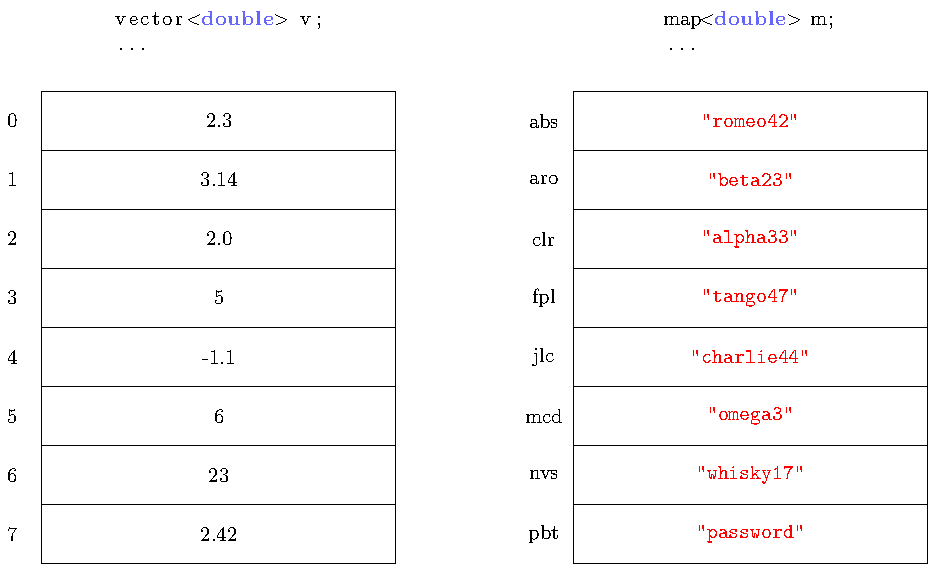
\includegraphics[height=4cm]{pics/cont.pdf}}
\end{center}
\end{frame}

\begin{frame}
\frametitle{Conteneurs séquentiels}
\begin{itemize}[<+->]
\item Les données sont parcourues selon l'ordre de rangement
\item Cet ordre dépend de la logique du conteneur
	\begin{itemize}
	\item Ordre d'ajout,
	\item Ordre croissant, etc.
	\end{itemize}
\item Pour accéder à un élément, il est nécessaire de spécifier un emplacement mémoire
	\begin{itemize}
	\item À la fin
	\item En troisième position
	\item Après un autre élément
	\end{itemize}
\end{itemize}
\begin{exampleblock}<+->{Exemple de conteneurs séquentiels}
	\begin{itemize}[<+->]
	\item Tableau : \texttt{array} et \texttt{vector}
	\item Liste doublement chaînée : \texttt{list}
	\item Liste chaînée de tableaux de taille fixé (compromis) : \texttt{deque}
	\end{itemize}
\end{exampleblock}
\end{frame}

\begin{frame}
\frametitle{Conteneurs associatifs}
\begin{itemize}[<+->]
\item Souvent mis en œuvre à l'aide de tableaux associatifs et de fonctions de hachage
	\begin{itemize}
	\item Tableau associatif : les clés sont triées selon leur ordre «~naturel~»
	\item Fonction de hachage : les clés sont triées selon la sortie de la fonction de hachage
	\end{itemize}
\item L'ajout et l'accès nécessitent une clé, pas un emplacement mémoire
	\begin{itemize}
	\item L'élément associé à \texttt{abs} est \lstinline|"romeo42"|
	\end{itemize}
\end{itemize}
\begin{exampleblock}<+->{Exemple de conteneurs associatifs}
	\begin{itemize}[<+->]
	\item Tableau de associatif : \texttt{map}
	\item Table de hachage : \texttt{unordered\_map}
	\item Ensembles : \texttt{set}, \texttt{unordered\_set}
	\end{itemize}
\end{exampleblock}
\end{frame}

\begin{frame}
\frametitle{Opérations courantes}
\begin{itemize}[<+->]
\item Ajout d'un élément
\item Suppression d'un élément
\item Contrôle de bornes
\item Itération
\item Algorithmique
	\begin{itemize}
	\item Tri de conteneurs séquentiels
	\item Fusion de séquences triées
	\item Recherche d'un élément
	\item Calcul du maximum
	\item Comparaisons lexicographiques
	\end{itemize}
\item Application de fonctions à tous les éléments
\end{itemize}
%\begin{alertblock}<+->{Remarque}
%	\begin{itemize}[<+->]
%	\item Attention à la complexité algorithmique
%	\item Choisir son conteneur en fonction de ses besoins
%	\end{itemize}
%\end{alertblock}
\end{frame}

\begin{frame}
\frametitle{Construction, copie et destruction}
\begin{itemize}[<+->]
\item Construire un conteneur d'objets entraîne pour chacun de ses éléments soit
	\begin{itemize}
	\item l'appel du constructeur par défaut 
	\item l'appel du constructeur de recopie
	\end{itemize}
\end{itemize}
\begin{exampleblock}<+->{Exemple}
	\begin{itemize}[<+->]
	\item \lstinline|vector<point> v(3);| : constructeur par défaut de \texttt{point}
	\item \lstinline|vector<point> w(v);| : constructeur de recopie de \texttt{vector<point>} qui appelle le constructeur de recopie de \texttt{point}
	\end{itemize}
\end{exampleblock}
\begin{itemize}[<+->]
\item La destruction d'un conteneur entraîne la destruction de ses éléments
	\begin{itemize}
	\item Si allocation dynamique : destruction «~manuelle~» nécessaire
	\end{itemize}
\end{itemize}
%\begin{itemize}[<+->]
%\item Par défaut, les conteneurs sont transmis par valeur en argument de fonction
%	\begin{itemize}
%	\item Coûteux : éviter
%	\end{itemize}
%\end{itemize}
\end{frame}

\begin{frame}
\frametitle{Remarques}
\begin{itemize}[<+->]
\item Chaque conteneur a ses propres performances
	\begin{itemize}
	\item Ajout, suppression, recherche
	\end{itemize}
\item La complexité algorithmique est précisée dans la documentation
\item Il faut donc choisir \emph{judicieusement} son conteneur en fonction des besoins
\item Les conteneurs sont amenés à allouer des espaces mémoires
	\begin{itemize}
	\item Spécifié par un allocateur
	\item Par défaut, les données sont souvent allouées dynamiquement
	\end{itemize}
\item Passer un conteneur par valeur (paramètre et retour) entraîne des copies
	\begin{itemize}
	\item Utiliser le passage par référence ou par adresse
	\item Utiliser le passage par sémantique de mouvement (cf. Ch. 9)
	\end{itemize}
\end{itemize}
\end{frame}

\begin{frame}
\frametitle{Construction, copie, affectation et destruction (2/2)}
\begin{itemize}[<+->]
\item La destruction d'un conteneur entraîne la destruction de ses éléments
	\begin{itemize}
	\item Si allocation dynamique : destruction «~manuelle~» nécessaire
	\end{itemize}
%\item Affectation \texttt{w = v} : comportement dépendant des tailles de \texttt{w} et \texttt{v}
%	\begin{itemize}
%	\item Si \texttt{w} est plus grand que \texttt{v} : affecte les éléments de \texttt{v} aux éléments de \texttt{w}, destruction des éléments excédentaires
%	\item Sinon, destruction des éléments de \texttt{w}, création d'un nouveau conteneur qui appelle le constructeur de recopie des éléments de \texttt{v}
%	\end{itemize}
\end{itemize}
\begin{alertblock}<+->{Remarque}
	\begin{itemize}[<+->]
	\item Prenez des précautions lors de l'utilisation de conteneurs
		\begin{itemize}
		\item Temps, mémoire
		\item Allocations dynamiques
		\end{itemize}
	\end{itemize}
\end{alertblock}
\end{frame}

\begin{frame}[containsverbatim]
\frametitle{Exemple 1}
\begin{itemize}
\item Fichier \texttt{cont-intro.cpp}
\end{itemize}
\begin{lstlisting}
class A
{
	int i;

	public:
		A(int i = 0) : i(i) { cout << "Builing " << this << endl; }
		
		A(const A& a) : i(a.i) { cout << "Copying " << &a << " into " << this << endl; }
		
		~A() { cout << "Destroying " << this << endl; }
		
		A& operator =(const A& a) //to track affectation
		{ 
			cout << "Affecting " << &a << " into " << this << endl;
			i = a.i;
			return *this;
		}		
};

void f(vector<A> v) { cout << "Entering f" << endl; }
\end{lstlisting}
\end{frame}

\begin{frame}[containsverbatim]
\frametitle{Exemple 1}
\begin{itemize}
\item Fichier \texttt{cont-intro.cpp}
\end{itemize}
\begin{lstlisting}
int main()
{	
	vector<A> v(3); cout << endl;

	vector<A> w(v); cout << endl;

	f(v);//passed by value
	cout << endl;

	vector<A*> y;
	for(int i = 0; i < 4; i++)
		y.push_back(new A(i));
	cout << endl;

	//memory leak here		
}
\end{lstlisting}
\end{frame}

\begin{frame}[containsverbatim]
\frametitle{Exemple 2}
\begin{itemize}
\item Fichier \texttt{cstr-def.cpp}
\end{itemize}
\begin{lstlisting}
class point
{
	int x, y;

	public:
		point(int x, int y) : x(x), y(y) 
        { 
            cout << "Building (" << x << "," << y << ")" << endl;
        }
};

int main()
{
	vector<point> v(3);
}
\end{lstlisting}
\end{frame}

\section{Itérateurs}

\begin{frame}
\frametitle{Généralités}
\begin{itemize}[<+->]
\item Objets permettant de parcourir le contenu d'un conteneur
	\begin{itemize}
	\item Bouche «~foreach~», etc.
	\end{itemize}
\item Utilisé régulièrement par la librairie sous la forme d'intervalle
	\begin{itemize}
	\item Exemple : recherche d'un élément dans une partie du conteneur
	\end{itemize}
\item Existe sur tous les conteneurs
\item Accès aux données via déférencement
\end{itemize}
\begin{exampleblock}<+->{Deux types de parcours}
	\begin{enumerate}[<+->]
	\item Parcours « standard » : obtenus via \texttt{begin()} et \texttt{end()}
	\item Parcours inverse : obtenus via \texttt{rbegin()} et \texttt{rend()}
	\end{enumerate}
\end{exampleblock}
\end{frame}

\begin{frame}
\frametitle{Initialisation : schéma}
\begin{center}
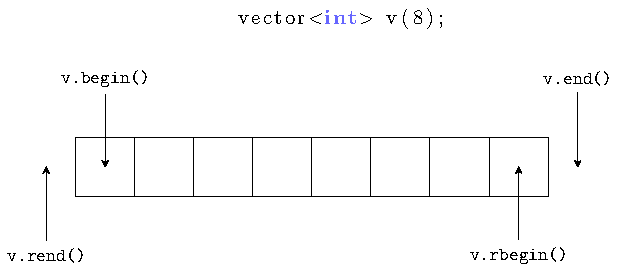
\includegraphics[width=12cm]{pics/iterator.pdf}
\end{center}
\end{frame}

\begin{frame}[containsverbatim]
\frametitle{Parcours : exemple}
\begin{itemize}
\item Fichier \texttt{iterate.cpp}
\end{itemize}
\begin{lstlisting}
int main()
{
	vector<int> v;
	v.push_back(1); v.push_back(2); v.push_back(3);
	vector<int>::iterator i;
	for(i = v.begin(); i != v.end(); i++)
		cout << *i << " ";
	cout << endl;

	for(int elem : v)
		cout << elem << " ";
	cout << endl;
}
\end{lstlisting}
\end{frame}

\begin{frame}
\frametitle{Intervalle d'itérateurs}
\begin{itemize}[<+->]
\item Permet de spécifier un intervalle d'itérateurs pour un algorithme
\item Toujours de la forme $[i,j[$
	\begin{itemize}
	\item Pratique au vu de l'initialisation
	\end{itemize}
\end{itemize}
\begin{exampleblock}<+->{Exemple}
	\begin{itemize}[<+->]
	\item Chercher un élément dans $\big[$\texttt{v.begin()}, \texttt{v.end()}$\big[$
	\end{itemize}
\end{exampleblock}
\begin{itemize}[<+->]
\item On suppose que $j$ soit «~atteignable~» à partir de $i$
\item Très utilisé dans  \texttt{algorithm.h}
\end{itemize}
\end{frame}

\begin{frame}[containsverbatim]
\frametitle{Exemple}
\begin{itemize}
\item Fichier \texttt{alg.cpp}
\end{itemize}
\begin{lstlisting}
int main()
{
	vector<int> v = {5,6,3,3,4,1,2};
	list<int> l;	

	copy(v.begin(), v.end(), back_inserter(l));
	cout << "list = ";
	for(int e : l)
		cout << e << " ";
	cout << endl << endl;

	equal(v.begin(),v.end(),l.begin()) ? cout << "true" : cout << "false";

	cout << count(v.begin(),v.end(), 3) << endl;

	auto i = find(v.begin(), v.end(), 3);
	cout << *i << endl;

	sort(v.begin(), v.end());
	for(int e : v)
		cout << e << " ";

	for_each(v.begin(), v.end(), [](int i) { cout << "Hello " << i << endl; } );
}
\end{lstlisting}
\end{frame}

\section{Conteneurs séquentiels}

\begin{frame}
\frametitle{Introduction}
\begin{itemize}[<+->]
\item Ordonnés explicitement par le programme
	\begin{itemize}
	\item \lstinline|v[1]| dénote le deuxième élément de \texttt{v}
	\end{itemize}
\item Différent des conteneurs associatifs
	\begin{itemize}
	\item Triés intrinsèquement par les clés ou une fonction de hachage
	\end{itemize}
\item Principaux représentants
	\begin{enumerate}
	\item \texttt{array<T,N>} : tableau de taille \texttt{N} fixe
	\item \texttt{vector<T>} : tableau de taille dynamique
	\item \texttt{list<T>} : liste doublement chaînée
	\item \texttt{deque<T>} : liste doublement chaînée de tableaux de tailles fixes
	\end{enumerate}
\item Performance des opérations varie en fonction du type de conteneur
\end{itemize}
\begin{exampleblock}<+->{Conclusion}
	\begin{itemize}[<+->]
	\item Choisir son conteneur en fonction de ses besoins
	\end{itemize}
\end{exampleblock}
\end{frame}

\begin{frame}
\frametitle{Construction}
\begin{itemize}[<+->]
\item Trois types de constructeurs de base pour \texttt{vector}, \texttt{list} et \texttt{deque}
	\begin{enumerate}
	\item Vide (par défaut)
	\item Nombre d'éléments (identiques) donnés
	\item Intervalle d'itérateurs
	\end{enumerate}
\item Pour \texttt{array}, seule la liste d'initialisation est autorisée
\end{itemize}
\begin{exampleblock}<+->{Exemple}
	\begin{enumerate}[<+->]
	\item \lstinline|array<int,4> a = \{3, 1, 2, 5\};|
	\item \lstinline|vector<int> v;|
	\item \lstinline|list<int> l(5);|
		\begin{itemize}
		\item Pas \lstinline|list<int> l = 5;| (constructeur \lstinline|explicit|)
		\item \lstinline|deque<point> dq (5, point(2,1));|
		\end{itemize}
	\item \lstinline|vector<int> v(l.begin(), l.end());|
	\end{enumerate}
\end{exampleblock}
\end{frame}

\begin{frame}
\frametitle{Affectation, recopie et destruction}
\begin{itemize}[<+->]
\item L'implémentation des conteneurs passe souvent par une allocation dynamique de mémoire
	\begin{itemize}
	\item Pas \texttt{array}
	\end{itemize}
\item Ils surchargent l'affectation et implémentent la recopie et destruction convenablement
\item Pour l'affectation et la recopie : le type \emph{doit} être identique
	\begin{itemize}
	\item Y compris dans les paramètres templates
	\end{itemize}
\end{itemize}
\begin{exampleblock}<+->{Exemple}
	\begin{itemize}[<+->]
	\item \lstinline|vector<int> vi1 ( ...), vi2 (...);|
	\item \lstinline|vector<double> vd1 (...);|
	\item \lstinline|vi1 = vi2; //ok| \hspace*{0.5cm} \lstinline|vd1 = vi1; //ko|
	\end{itemize}
\end{exampleblock}
\end{frame}

\begin{frame}
\frametitle{Autres fonctions globales}
\begin{itemize}[<+->]
\item \texttt{swap} échange le contenu de deux conteneurs
	\begin{itemize}
	\item \texttt{v1.swap(v2);}
	\item Plus efficace qu'un \texttt{swap} manuel
	\end{itemize}
\item \texttt{clear}
	\begin{itemize}
	\item Taille nulle après \texttt{v.clear();} (pas avec \texttt{array})
	\item Appelle les destructeurs
	\end{itemize}
\item Opérateur \texttt{==} et \texttt{<}
	\begin{itemize}
	\item Comparaison lexicographique, éléments comparés 2 à 2
	\item Les objets doivent surcharger \texttt{==} ou \texttt{<}
	\end{itemize}
\end{itemize}
\end{frame}

\begin{frame}[containsverbatim]
\frametitle{Exemple}
\begin{itemize}
\item Fichier \texttt{other.cpp}
\end{itemize}
\begin{lstlisting}
int main()
{
	vector<int> v1 = {1,2,3,6};
	vector<int> v2 = {2,3,4,5,0};

	cout << ((v1 < v2) ? "v1 < v2" : "v2 >= v1") << endl;

	v1.swap(v2);
	for_each(v1.begin(), v1.end(), [](int& i) { cout << i << " "; }); 
	cout << endl;
	for_each(v2.begin(), v2.end(), [](int& i) { cout << i << " "; }); 
	cout << endl;

	point p1(1,1);
	point p2(2,2);
	vector<point> vp1; vp1.push_back(p1); vp1.push_back(p2);
	vector<point> vp2; vp2.push_back(p1); vp2.push_back(p2);	
	cout << ((vp1 == vp2) ? "vp1 == vp2" : "vp1 != vp2") << endl;

	vp1.clear();
}
\end{lstlisting}
\end{frame}

\begin{frame}
\frametitle{Insertion et suppression}
\begin{itemize}[<+->]
\item \texttt{vector}, \texttt{list} et \texttt{deque} offrent la possibilité d'ajouter et supprimer des éléments
	\begin{itemize}
	\item Au début, à la fin ou sur une position arbitraire
	\item Fonctions \texttt{push\_back}, \texttt{pop\_back}, \texttt{push\_front}, \texttt{pop\_front}, \texttt{insert}, \texttt{erase}
	\end{itemize}
\item Performances varient fortement en fonction du type de conteneur et de l'emplacement
\item Ajout
	\begin{itemize}
	\item \texttt{vector} : $\bigo(1)$ à la fin «~s'il reste de la place~», $\bigo(n)$ sinon
	\item \texttt{deque} : $\bigo(1)$ au début ou à la fin «~s'il reste de la place~», $\bigo(n)$ sinon
	\item \texttt{list} : $\bigo(1)$ au début, à la fin et «~sur un itérateur~»
	\end{itemize}
\item Suppression
	\begin{itemize}
	\item \texttt{vector} : $\bigo(1)$ à la fin, $\bigo(n)$ sinon
	\item \texttt{deque} : $\bigo(1)$ au début ou à la fin, $\bigo(n)$ sinon
	\item \texttt{list} : $\bigo(1)$ au début, à la fin et «~sur un itérateur~»
	\end{itemize}
\end{itemize}
\end{frame}

\begin{frame}[containsverbatim]
\frametitle{Exemple}
\begin{itemize}
\item Fichier \texttt{insert-erase.cpp}
\end{itemize}
\begin{lstlisting}
int main()
{
	list<double> l = {2.5, 3.5, 6.5, 7.5};

	auto it1 = l.begin(); it1++; it1++;
	l.insert(it1, 1.5); l.insert(it1, 10, -1); //what is l ?

	vector<double> v = {1.1, 2.2, 3.3};
	it1++;it1++;it1++;
	l.insert(it1, v.begin(), v.end()); //what is v ?

	it1 = l.begin();
	for(int i = 0; i < 5; i++)
		it1++;
	l.insert(it1, v.begin(), v.end()); //what is l ?

	it1 = l.begin();
	auto it2 = l.end(); it2--; it2--;
	for(int i = 0; i < 9; i++)
		it1++;
	l.erase(it1, it2); //what is l ?
}
\end{lstlisting}
\end{frame}

\begin{frame}
\frametitle{Invalidation d'itérateurs}
\begin{itemize}[<+->]
\item Modifier le contenu d'un conteneur quand des itérateurs y sont instanciés peuvent les \emph{invalider}
\item Le comportement de l'itérateur n'est pas celui attendu
	\begin{itemize}
	\item Souvent, comportement indéterminé (déférencement, déplacement)
	\end{itemize}
\item Invalidations précisées dans la documentation
	\begin{itemize}
	\item Avec \texttt{array}, pas d'invalidation possible
	\end{itemize}
\end{itemize}
\begin{exampleblock}<+->{Exemple : \texttt{vector}}
	\begin{itemize}[<+->]
	\item Invalidés sur tous les éléments si augmentation de taille
	\item Tous les éléments «~suivants~» si suppression
	\end{itemize}
\end{exampleblock}
\begin{itemize}[<+->]
\item En \java, lancement d'une exception
\end{itemize}
\end{frame}

\begin{frame}
\frametitle{Accès aux éléments}
\begin{itemize}
\item Performances varient fortement en fonction
	\begin{itemize}
	\item du type de conteneur
	\item de l'emplacement
	\end{itemize}
\end{itemize}
\begin{exampleblock}<+->{Complexité}
	\begin{itemize}[<+->]
	\item \texttt{vector} et \texttt{array} : $\bigo(1)$ dans tous les cas
	\item \texttt{list} : $\bigo(1)$ au début et à la fin, $\bigo(n)$ sinon
	\item \texttt{deque} : $\bigo(1)$ dans tous les cas (moins bon que \texttt{vector})
	\end{itemize}
\end{exampleblock}
\begin{itemize}
\item Opérateur \texttt{[]} (pas de contrôle de borne) ou fonction \texttt{at} pour \texttt{array}, \texttt{vector} et \texttt{deque}
\item Pour \texttt{list}, on accède à un élément via un itérateur
\end{itemize}
\end{frame}

\begin{frame}[containsverbatim]
\frametitle{Exemple}
\begin{itemize}
\item Fichier \texttt{acces.cpp}
\end{itemize}
\begin{lstlisting}
int main()
{
    array<int,5> a = {1, 1, 2, 3, 5};
	vector<int> v = {1, 2, 3, 4, 5};
	list<int> l = {5, 6, 7, 8};
	deque<int> d = {10, 11, 12, 13, 14};

	for(int i = 0; i < 4; i++)
		cout << a[i] << " " << v[i] << " " << d[i] << endl;
	cout << endl;

	cout << l.front() << endl;	
	cout << l.back() << endl;

	auto it = l.begin();
	it++;
	cout << *it << endl;
	it++;
	cout << *it << endl;
}
\end{lstlisting}
\end{frame}

\begin{frame}
\frametitle{Augmentation de taille d'un \texttt{vector}}
\begin{itemize}[<+->]
\item Trois attributs particuliers dans \texttt{vector}
	\begin{enumerate}
	\item \texttt{size()} : nombre d'éléments stockés
	\item \texttt{capacity()} : nombre d'éléments stockables sans augmentation de taille
	\item \lstinline|max_size()| : nombre maximum d'éléments stockables
	\end{enumerate}
\item On a toujours \lstinline|size()| $\leqslant$ \lstinline|capacity()| $\leqslant$ \lstinline|max_size()|
\end{itemize}
\begin{exampleblock}<+->{Ajout d'éléments}
	\begin{itemize}[<+->]
	\item Si \lstinline|size()| $<$ \lstinline|capacity()| : $\bigo(1)$
	\item Sinon
		\begin{enumerate}
		\item Création d'un tableau de taille double (\lstinline|capacity()| $\times 2$)
		\item Recopie des éléments du «~petit~» tableau ($\bigo(n)$)
		\item Destruction du petit tableau
		\end{enumerate}
	\end{itemize}
\end{exampleblock}
\begin{itemize}[<+->]
\item Même comportement pour \texttt{std::string}
\end{itemize}
\end{frame}

\begin{frame}[containsverbatim]
\begin{itemize}
\item Fichier \texttt{vect-capac-increase.cpp}
\end{itemize}
\begin{lstlisting}
int main()
{	
	vector<int> v(3);
	cout << "size = " << v.size() << " , capacity = " << v.capacity() << endl;
	for(int i = 0; i < 20 ; i++)
	{
		v.push_back(2);
		cout << "size = " << v.size() << " , capacity = " << v.capacity() << endl;
	}
	cout << endl;	

	v = vector<int>(3);
	v.reserve(5);
	cout << "size = " << v.size() << " , capacity = " << v.capacity() << endl << endl;

	v = vector<int>(3);
	v.push_back(2);
	v.reserve(5);
	cout << "size = " << v.size() << " , capacity = " << v.capacity() << endl << endl;
	
	cout << v.max_size() << endl;
}
\end{lstlisting}
\end{frame}

\section{Adaptateurs}

\begin{frame}
\frametitle{Généralités}
\begin{itemize}[<+->]
\item Conteneur aux propriétés d'ajout et d'accès particulières
\item Implémentation non imposée par le standard
\end{itemize}
\begin{exampleblock}<+->{Opérations}
	\begin{itemize}[<+->]
	\item Ajout d'un élément (sans choisir «~où~»)
	\item Accès d'un élément (sans choisir «~où~»)
	\end{itemize}
\end{exampleblock}
\begin{itemize}[<+->]
\item Trois adaptateurs
	\begin{enumerate}
	\item \texttt{stack} : pile (LIFO)
	\item \texttt{queue} : file (FIFO)
	\item \lstinline{priority_queue} : file à priorité (\texttt{<})
	\end{enumerate}
\end{itemize}
\end{frame}

\begin{frame}
\frametitle{Adaptateur \lstinline|stack|}
\begin{itemize}[<+->]
\item Fournit une structure de donnée LIFO
\item Construit par défaut ou sur base d'un conteneur séquentiel
	\begin{itemize}
	\item Pour un usage exclusif, utilisez \texttt{list}
	\item Efficace
	\end{itemize}
\end{itemize}
\begin{exampleblock}<+->{Opérations}
	\begin{itemize}[<+->]
	\item \lstinline|push| : met un élément au sommet de la pile
	\item \lstinline|pop| : supprime l'élément au sommet de la pile
	\item \lstinline|top| : accède au sommet de la pile
	\end{itemize}
\end{exampleblock}
\end{frame}

\begin{frame}
\frametitle{Illustration}
\begin{center}
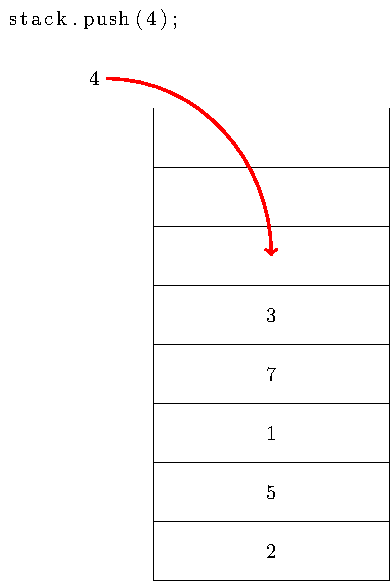
\includegraphics[height=6cm]{pics/stack-1.pdf}
\hspace{2cm}
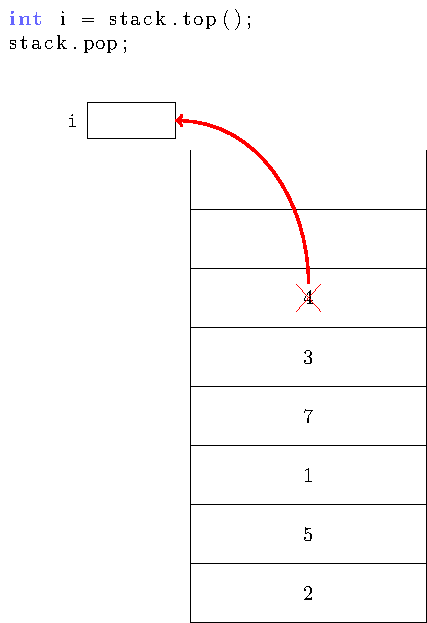
\includegraphics[height=6cm]{pics/stack-2.pdf}
\end{center}
\end{frame}

\begin{frame}[containsverbatim]
\begin{itemize}
\item Fichier \texttt{stack.cpp}
\end{itemize}
\begin{lstlisting}
int main()
{	
	stack<int> q;

	for(int i = 0; i < 10; i++)
		q.push(i * i);

	while(! q.empty())
	{
		cout << q.top() << " ";
		q.pop();
	}
	cout << endl;
	
	for(int i = 0; i < 10; i++)
		q.push(i * i);
	q.top() = 99;
		
	for(int i = 0; i < q.size(); i++)//sneaky loop is sneaky
	{
		cout << q.top() << " ";
		q.pop();
	}
	cout << endl << q.size() << endl;
}
\end{lstlisting}
\end{frame}

\begin{frame}
\frametitle{Adaptateur \lstinline|queue|}
\begin{itemize}[<+->]
\item Fournit une structure de donnée FIFO
\item Construit par défaut ou sur base d'un conteneur séquentiel
	\begin{itemize}
	\item Pour un usage exclusif, utilisez \texttt{list}
	\item Efficace
	\end{itemize}
\end{itemize}
\begin{exampleblock}<+->{Opérations}
	\begin{itemize}[<+->]
	\item \lstinline|push| : met un élément à la fin de la file
	\item \lstinline|pop| : supprime l'élément au début de la file
	\item \lstinline|front| : accède au début de la file
	\item \lstinline|back| : accède à la fin de la file
	\end{itemize}
\end{exampleblock}
\end{frame}

\begin{frame}[containsverbatim]
\begin{itemize}
\item Fichier \texttt{queue.cpp}
\end{itemize}
\begin{lstlisting}
int main()
{	
	queue<int> q;	

	for(int i = 0; i < 10; i++)
		q.push(i * i);

	q.front() = 99;
	q.back() = -99;

	while(! q.empty())
	{
		cout << q.front() << " ";
		q.pop();
	}
	cout << endl;
}
\end{lstlisting}
\end{frame}

\begin{frame}
\frametitle{Adaptateur \lstinline|priority_queue|}
\begin{itemize}[<+->]
\item Permet de maintenir un ordre sur les éléments
	\begin{itemize}
	\item Opérateur \texttt{<} : «~priorité~»
	\item Possibilité de fournir un comparateur par surcharge d'opérateur (Cf. Ch. 8)
	\end{itemize}
\item Construit par défaut ou sur base d'un conteneur séquentiel
	\begin{itemize}
	\item Pour un usage exclusif, utilisez \texttt{deque}
	\item Efficace
	\end{itemize}
\end{itemize}
\begin{exampleblock}<+->{Opérations}
	\begin{itemize}[<+->]
	\item \lstinline|push| : met un élément dans la file à priorité
	\item \lstinline|pop| : supprime l'élément de plus haute priorité
	\item \lstinline|top| : accède à l'élément de plus haute priorité
		\begin{itemize}
		\item Ne peut pas être réaffecté
		\end{itemize}
	\end{itemize}
\end{exampleblock}
\end{frame}

\begin{frame}[containsverbatim]
\frametitle{Exemple}
\begin{itemize}
\item Fichier \texttt{pqueue.cpp}
\end{itemize}
\begin{lstlisting}
int main()
{	
	priority_queue<int> q;
	
	for(int i = 0; i < 10; i++)
	{
		int r = rand() % 100 + 1;
		q.push(r);
		cout << "pushed " << r << endl;
	}	
	cout << endl;

	while(! q.empty())
	{
		cout << q.top() << " ";
		q.pop();
	}

	cout << endl;
}
\end{lstlisting}
\end{frame}

\section{Conteneurs associatifs}

\begin{frame}
\frametitle{Généralités}
\begin{itemize}[<+->]
\item Structure de données associant une «~clé~» à une valeur.
\item On accède aux valeurs via leur clé
	\begin{itemize}
	\item Identique pour la suppression
	\end{itemize}
\item Souvent mis en œuvre à l'aide de tableaux associatifs et de tables de hachage
	\begin{itemize}
	\item Tableau associatif : clés triées selon leur ordre «~naturel~»
	\item Table de hachage : clés triées avec la fonction de hachage
	\end{itemize}
\item Les éléments sont parcourus en suivant l'ordre des clés
\end{itemize}
\begin{exampleblock}<+->{Exemple}
	\begin{enumerate}[<+->]
	\item Tableaux associatifs : \texttt{map}, \texttt{multimap}, \texttt{set}, \texttt{multiset}
	\item Tables de hachage : \lstinline|unordered_map|, etc.
	\end{enumerate}
\end{exampleblock}
\end{frame}

\begin{frame}
\frametitle{Fonction de hachage : introduction}
\begin{itemize}[<+->]
\item Toute fonction associant un \emph{message} (clé) à un \emph{condensé}
	\begin{itemize}
	\item Les messages ont une forme arbitraire (chaînes de caractères, bytes, etc.)
	\item Souvent, les condensés sont naturels
	\end{itemize}
\end{itemize}
\begin{exampleblock}<+->{Exemple}
	\begin{itemize}
	\item \lstinline|int i = f("John smith"); //7|
	\end{itemize}
\end{exampleblock}
\begin{itemize}[<+->]
\item Habituellement, «~non inversibles~»
\item Si deux messages ont le même condensé : collision
\item Exemples de fonctions de hachage : \textsc{SHA-1}, \textsc{MD-5}
\item Domaine très important en informatique théorique
	\begin{itemize}
	\item Question à 1M\$ : «~Do one-way functions exist ?~»
	\end{itemize}
\end{itemize}
\end{frame}

\begin{frame}
\frametitle{Fonction de hachage : illustration}
\begin{center}
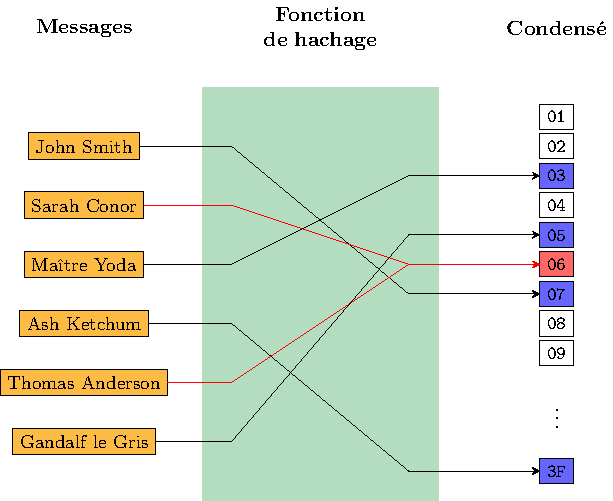
\includegraphics[width=7cm]{pics/hash.pdf}
\end{center}
\end{frame}

\begin{frame}
\frametitle{Le patron de classe \texttt{pair}}
\begin{itemize}[<+->]
\item Souvent, les «~tuples~» dans un conteneur associatifs sont stockés via \texttt{pair}
	\begin{itemize}
	\item Spécialisation de \texttt{tuple}
	\item Modélise une paire d'éléments de type donnés
	\end{itemize}	
\item Dispose d'opérateurs
	\begin{itemize}
	\item \texttt{==} et \texttt{!=} : comparaison de contenu
	\item \texttt{<} et associés : comparaison lexicographique
	\end{itemize}
\item Patron utile lors de parcours itératif de conteneur associatif
	\begin{itemize}
	\item «~Pour chaque paire de \texttt{brol,truc}~» au sein de la \texttt{map} \dots
	\end{itemize}
\item Fournit des conversions implicites
	\begin{itemize}
	\item Très rare dans les templates
	\item Souvent, utilisation de \lstinline|make_pair|
	\end{itemize}
\end{itemize}
\end{frame}

\begin{frame}[containsverbatim]
\frametitle{Exemple}
\begin{itemize}
\item Fichier \texttt{pair.cpp}
\end{itemize}
\begin{lstlisting}
int main()
{
	pair<int, float> p1;
	cout << "Init : " << p1.first << ", " << p1.second << endl;
 
	pair<int, double> p2(42, 0.123);
	cout << "Initialized :" << p2.first << ", " << p2.second << endl;
 
	pair<char, int> p3(p2);
	cout << "Implicitly converted: " << p3.first << ", " << p3.second << endl;

	int n = 1;
	int a[5] = {1, 2, 3, 4, 5};
 
	// build a pair from two ints
	auto p4 = make_pair(n, a[1]);
	cout << "The value of p3 is " << "(" << p4.first << ", " << p4.second << ")" << endl;
 
	// build a pair from a reference to int and an array (decayed to pointer)
	auto p5 = make_pair(ref(n), a);
	n = 7;
	cout << "The value of p4 is " << "(" << p5.first << ", " << *(p5.second + 1) << ")" 
		   << endl;
}
\end{lstlisting}
\end{frame}

\begin{frame}
\frametitle{Le conteneur \texttt{map}}
\begin{itemize}[<+->]
\item Dictionnaire associant une clé à une valeur
\end{itemize}
\begin{exampleblock}<+->{Opérations}
	\begin{itemize}[<+->]
	\item Ajout / suppression : $\bigo(\log(n))$ (\texttt{insert} et \texttt{erase})
	\item Accès : $\bigo(\log(n))$
	\end{itemize}
\end{exampleblock}
\begin{itemize}[<+->]
\item Les clés sont triées selon leur ordre naturel
	\begin{itemize}
	\item Opérateur \texttt{<}
	\item Possibilité de fournir un comparateur via surcharge d'opérateur (Cf. Ch. 8)
	\end{itemize}
\end{itemize}
\end{frame}

\begin{frame}[containsverbatim]
\frametitle{Exemple}
\begin{itemize}
\item Fichier \texttt{map.cpp}
\end{itemize}
\begin{lstlisting}
void print(const map<char, int> &m)
{
	cout << "Map : " << endl;
	for(auto e : m)
		cout << "( " << e.first << " , " << e.second << " )" << endl;
	cout << endl;
}

int main()
{
	map<char, int> m;
	print(m);

	m['S'] = 5; m['C'] = 10;
	m['s'] = 2;
	print(m);

	m['S'] = m['D'];
	print(m);
}
\end{lstlisting}
\end{frame}

\begin{frame}
\frametitle{Accès aux éléments}
\begin{itemize}
\item Accès via l'opérateur \texttt{[]}
\end{itemize}
\begin{alertblock}<+->{Remarque importante}
	\begin{itemize}[<+->]
	\item Pas de contrôle de bornes
	\item Si \texttt{m[i]} n'existe pas, il est créé
	\end{itemize}
\end{alertblock}
\begin{itemize}[<+->]
\item Fonction \texttt{at} : accès avec contrôle de bornes
	\begin{itemize}
	\item Un élément non existant n'est pas créé (exception)
	\end{itemize}
\item Accès par itérateur
	\begin{itemize}
	\item La fonction \texttt{find} retourne un itérateur sur un élément ayant une clé donnée, ou sur \texttt{end()} s'il n'existe pas
	\item Déférencement de \texttt{pair} via \texttt{*}
	\item Obtention des clés / valeurs via les attributs \texttt{first} et \texttt{second}
	\item Comportement de \lstinline|*it = make_pair('S', 5);| non spécifié
	\end{itemize}
\end{itemize}
\end{frame}

\begin{frame}[containsverbatim]
\frametitle{Exemple}
\begin{itemize}
\item Fichier \texttt{map-access.cpp}
\end{itemize}
\begin{lstlisting}
int main()
{	
	map<int, float> m;

	for(int i = 0; i < 3; i++)
		m[i] = i + 0.5;

	cout << "m[5] = " << m[5] << endl;

	for(auto e : m)
		cout << "( " << e.first << " , " << e.second << " )" << endl;
	cout << endl;

	cout << (*m.find(2)).second << endl;
	
	if(m.find(6) != m.end())
		cout << (*m.find(6)).second << endl;
	else
		cout << "Key '6' does not exist" << endl;	
	
	for(auto e : m)
		cout << "( " << e.first << " , " << e.second << " )" << endl;
	cout << endl;
}
\end{lstlisting}
\end{frame}

\begin{frame}
\frametitle{Autres conteneurs (1/2)}
\begin{exampleblock}<+->{Conteneur \texttt{multimap}}
	\begin{itemize}[<+->]
	\item Conteneur à la signature identique à \texttt{map}, mais plusieurs valeurs peuvent être associées à une clé
	\item \texttt{find} fournit un itérateur sur l'un des éléments associés
		\begin{itemize}
		\item Pas nécessairement le premier
		\end{itemize}
	\item \lstinline|equal_range| fournit tous les éléments associés à une clé
	\item \texttt{erase} efface tous les éléments associés à une clé (ou intervalle)
	\end{itemize}
\end{exampleblock}
\begin{exampleblock}<+->{Conteneur \texttt{set}}
	\begin{itemize}[<+->]
	\item Conteneur identique à \texttt{map}, mais avec les clés uniquement
		\begin{itemize}
		\item Idée : liste triée d'éléments uniques
		\end{itemize}
	\item Les éléments sont constants
	\end{itemize}
\end{exampleblock}
\end{frame}

\begin{frame}
\frametitle{Autres conteneurs (2/2)}
\begin{itemize}[<+->]
\item \lstinline|multiset| : signature identique à \texttt{set}, mais les doublons sont autorisés
	\begin{itemize}
	\item Remarques identiques aux spécificités de \lstinline|multimap|
	\end{itemize}
\item \lstinline|unordered_map|, \lstinline|unordered_multimap|, \lstinline|unordered_set|
\lstinline|unordered_multiset|
	\begin{itemize}
	\item Même signature que les conteneurs associatifs associés, mais les clés sont spécifiés par une fonction de hachage
	\item Possibilité de spécifier sa fonction de hachage via un foncteur
	\end{itemize}
\end{itemize}
\begin{exampleblock}<+->{Remarque}
	\begin{itemize}[<+->]
	\item Créer une fonction de hachage ayant les propriétés désirées est parfois très difficile
	\end{itemize}
\end{exampleblock}
\end{frame}
\end{document}
